\section{Conceptos Fundamentales}

\begin{frame}
	\begin{block}{Conceptos Fundamentales}
		 \begin{enumerate}
		  \item Sistemas de gestión de flujos de trabajo científicos.
		  \item Sistemas de recomendación.
		  \item Recomendación sobre flujos de trabajo científicos.
		  \item Ontologías.
		  \item Recomendación basada en bases de datos de flujos de trabajo científicos.
		  \item Validación de métricas.
		  \item Recomendación de la base de datos de flujo de trabajo.
		  \item Clasificadores y regresores.
		 \end{enumerate}
	\end{block}
\end{frame}


\begin{frame}
	\begin{figure}[!htb]
		\centering	  				
		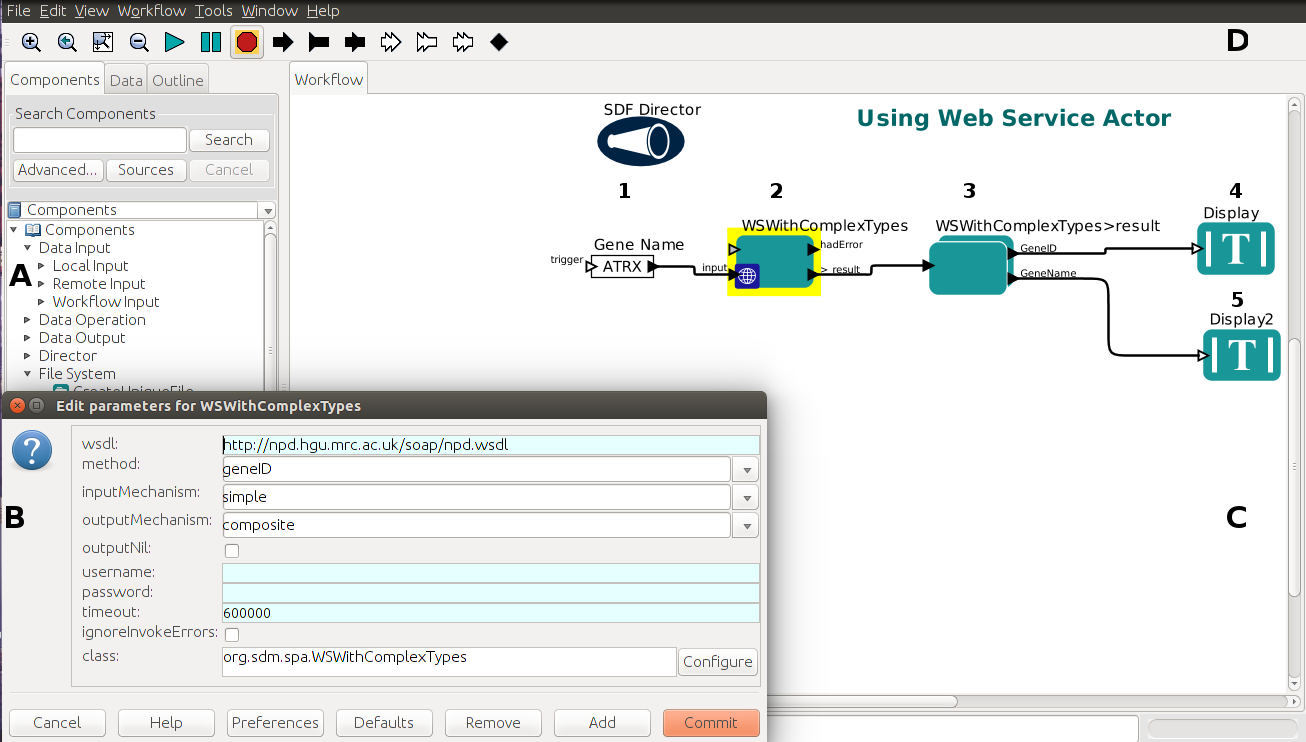
\includegraphics[height=7cm]{./secoes/ConceitosFundamentais/webService.png}
		\caption{Ejemplo de sistema de gestión de flujo de trabajo científico.}
		\label{fig_sistema_gerenciador_workflow_cientifico}
 	\end{figure}
\end{frame}


\begin{frame}		
	\begin{block}{}
		Los sistemas de recomendación están destinados a \textbf{recomendar elementos útiles} a los usuarios:
		\begin{eqnarray}
		\forall c \in C,  \quad s_{c}^{'} =  \operatorname*{arg\,max}_{s \in S} u(c,s) \label{formalizar_recomendacao}
		\end{eqnarray}
		
%		A função utilidade \(u\) não está definida para todo o espaço \(C \times S\), isso força os sistemas de recomendação a extrapolar o espaço conhecido.
		La función de utilidad \(u\) no está definida para todo el espacio \(C \times S\), esto obliga a los sistemas de recomendación a extrapolar el espacio conocido.
	\end{block}
\end{frame}


\begin{frame}
	\begin{block}{}
		Algunas estrategias utilizadas en los sistemas de recomendación:
		
		\begin{enumerate}
			\item \emph{Content-based}
			\item \emph{Collaborative Filter (usuarios similares)}
			\item \emph{Hibrid Approach}
			\item \emph{Community Based (usuarios amigables)}
			\item \emph{Demographic}
			\item \emph{Knowledge-based}
		\end{enumerate}
	\end{block}
\end{frame}


\begin{frame}		
	\begin{block}{}
		\textbf{Recomendar actividades en flujos de trabajo científicos} requiere, además de la extrapolación mencionada anteriormente, considerar las restricciones:
		\begin{enumerate}
			\item Dependencia entre entrada y salida de actividades
			\item Dependencia semántica
			\item El orden de las actividades
		\end{enumerate}
	\end{block}
\end{frame}


\begin{frame}
	\begin{block}{}
		\textbf{Ontology} es un modelo para la representación del conocimiento, que se puede utilizar para anotar semánticamente actividades.
		
		\begin{figure}
			\begin{minipage}[b]{0.7\textwidth}
				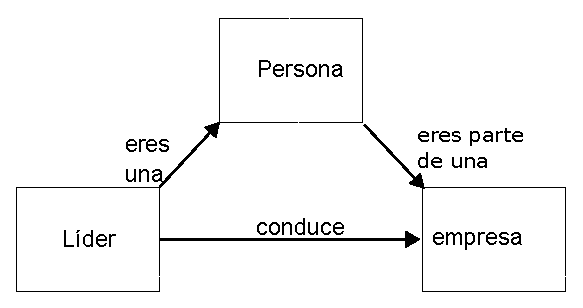
\includegraphics[width=\textwidth]{./secoes/ConceitosFundamentais/Ontologia.eps}
				\caption{Ejemplo de ontología}
			\end{minipage}
		\end{figure}
	\end{block}
\end{frame}

\begin{frame}
	\begin{block}{}
		Los experimentos serán validados por \emph{validación cruzada 10 veces}, cada ronda calculará las métricas:
		\begin{enumerate}
			\item \emph{Sucess at rank k} (\(S@k\)).
			\item \emph{Mean Reciprocal Rank} (MRR).		
		\end{enumerate}
		
		\begin{figure}
			\begin{minipage}[b]{0.9\textwidth}
				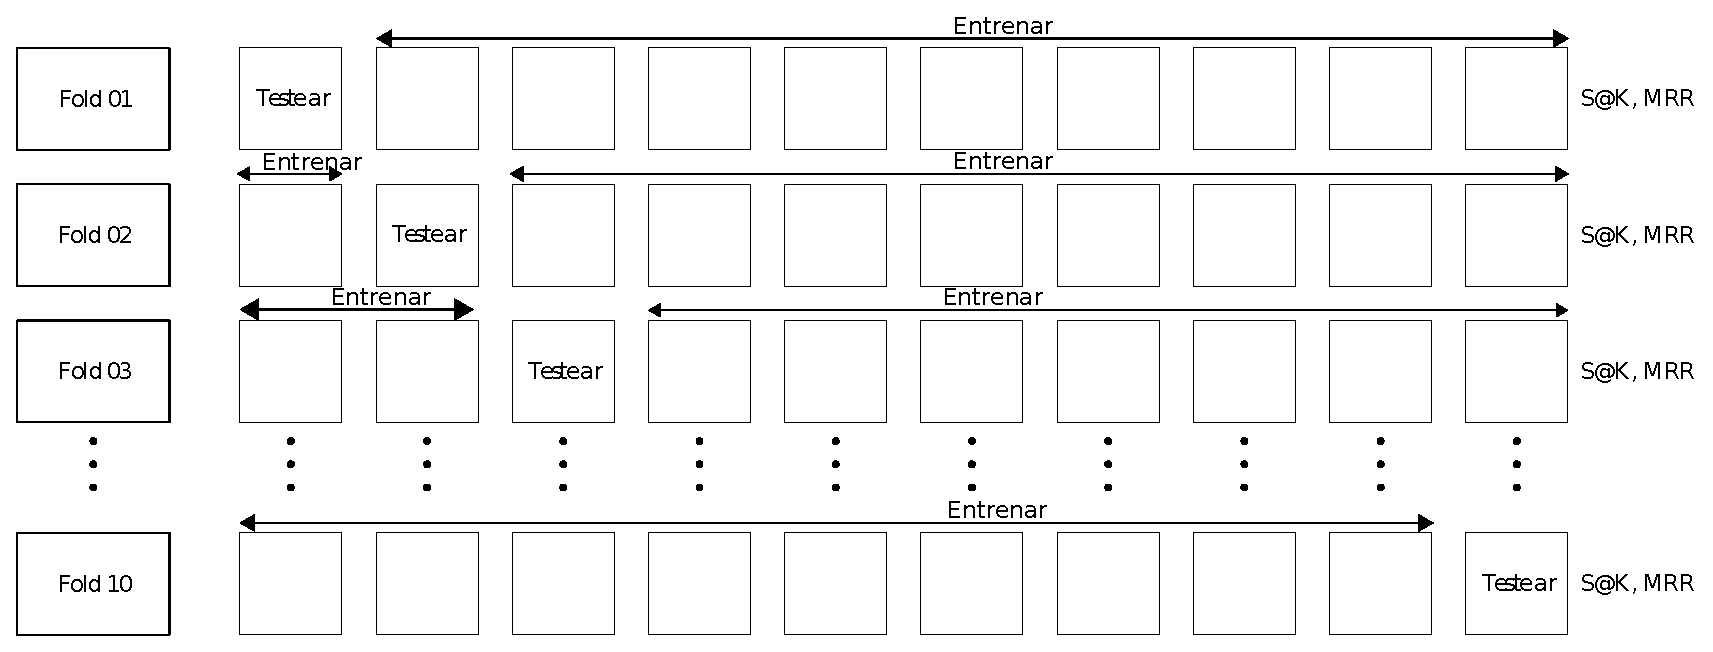
\includegraphics[width=\textwidth]{./secoes/ConceitosFundamentais/10FOLDCROSS.eps}
				\caption{Exemplo de \emph{10-fold cross validation}}
			\end{minipage}
		\end{figure}
		
	\end{block}
\end{frame}

\begin{frame}
	\begin{block}{}
		\textbf{Recomendación de base de datos de flujo de trabajo}
		\begin{enumerate}
			\item Frecuencia
			\item \emph{itemsets}.	
		\end{enumerate}
	\end{block}
\end{frame}


\begin{frame}
	\begin{block}{}
		\textbf{Recomendación de clasificadores}
		\begin{enumerate}
			\item CART;
			\item KNN;
			\item Naive Bayes;
			\item Rede Neural (MLP);
			\item SVM (C-SVM).		
		\end{enumerate}
	\end{block}
\end{frame}

\begin{frame}
	\begin{block}{}
		\textbf{Recomendación de los regresores}
		\begin{enumerate}
			\item CART;
			\item MARS;
			\item Binomial;
			\item Rede Neural (MLP);
			\item SVM (\(\epsilon\)-SVM).		
		\end{enumerate}
	\end{block}
\end{frame}

\begin{frame}
	\begin{block}{}
		\textbf{Recomendación de clasificadores compuestos}
		\begin{enumerate}
			\item SVM;
			\item Rotation Forest.		
		\end{enumerate}
	\end{block}
\end{frame}
